\begin{frame}\frametitle{Large Hadron Collider (LHC)}
%\begin{figure}[htb]
%  \begin{center}
%    {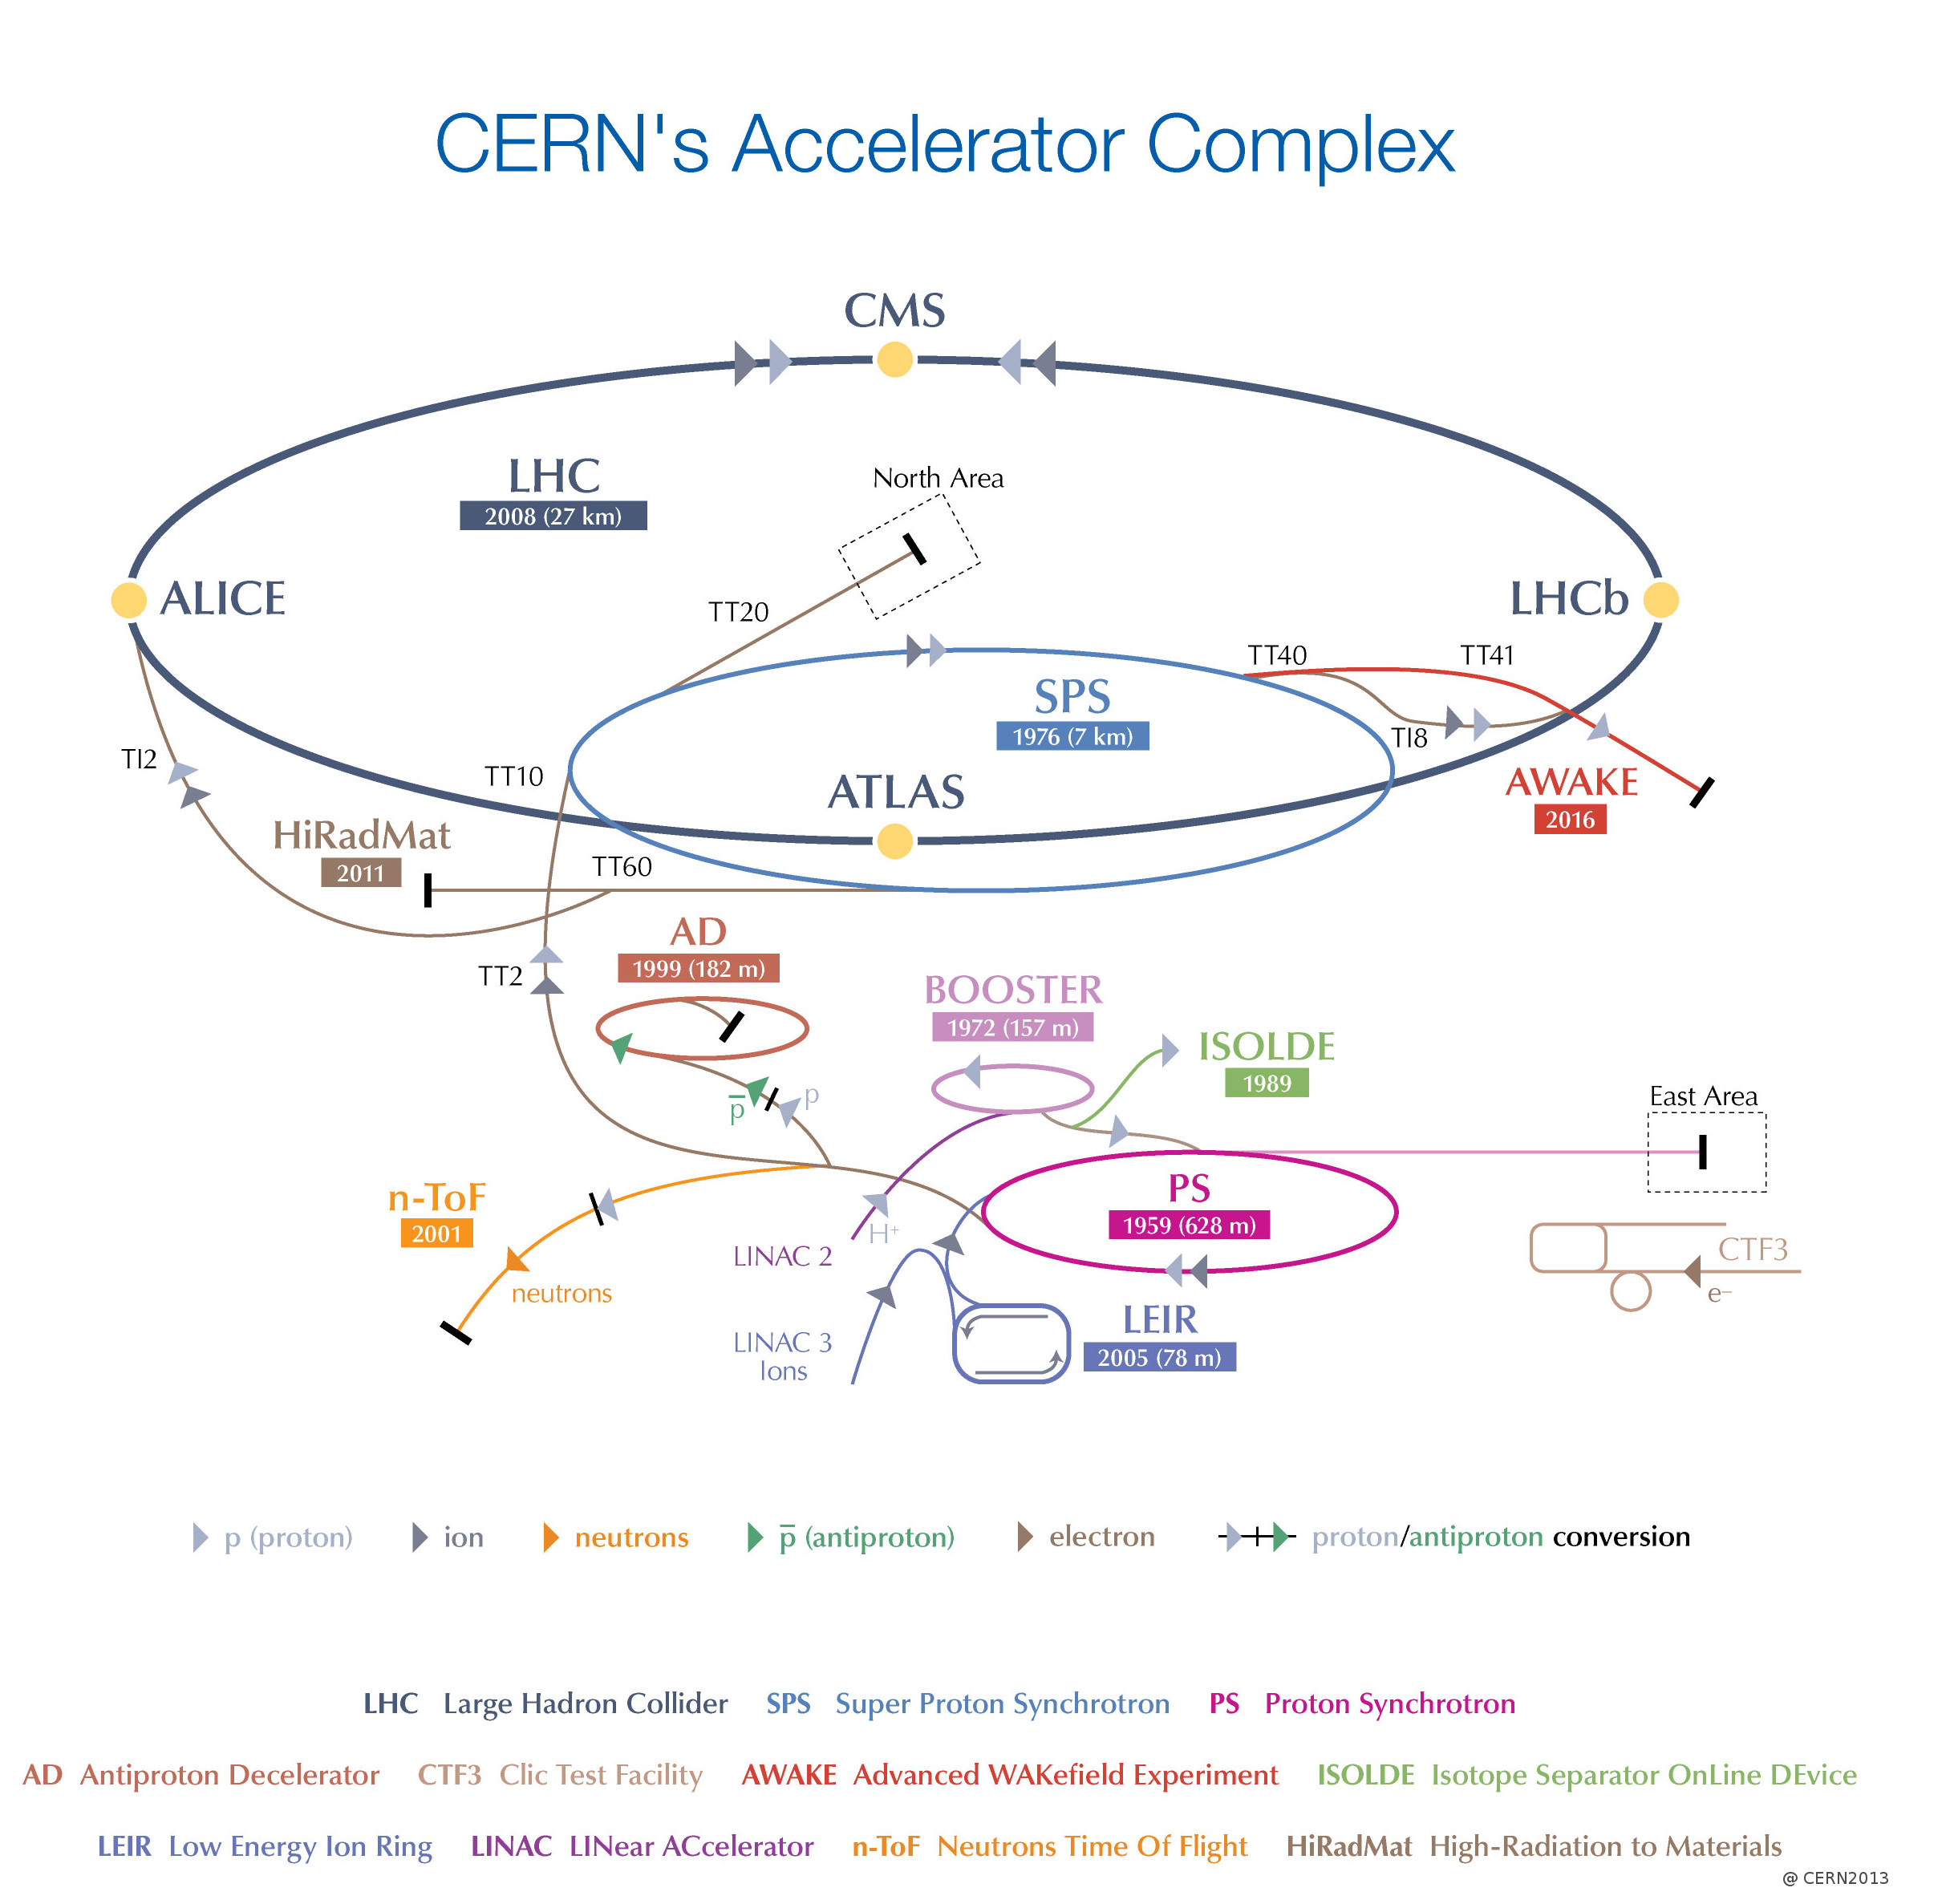
\includegraphics[width=0.80\textwidth]{../figs/Exp/CERN_accelerator_complex2013.jpg}}
%    \caption\tiny{CERN's accelerator complex~\cite{ref_fig_CERNacceleratorComplex}.}
%    \label{fig:CERN_accelerator_complex}
%  \end{center}
%\end{figure}
\end{frame}%{Large Hadron Collider}

\begin{frame}\frametitle{Compact Muon Solenoid (CMS). Components}
\begin{figure}[htb]
  \begin{center}
%    {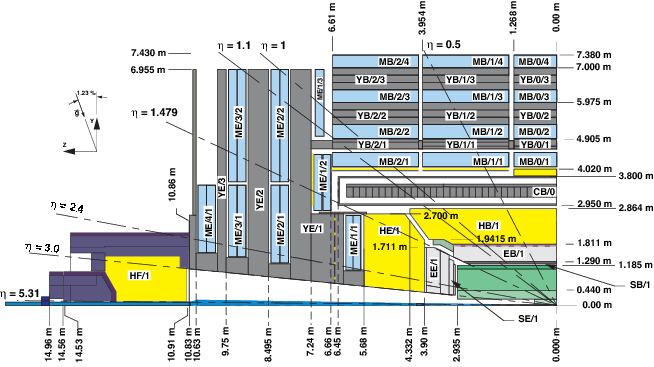
\includegraphics[width=0.45\textwidth]{../figs/Exp/CMSview1.png}
%     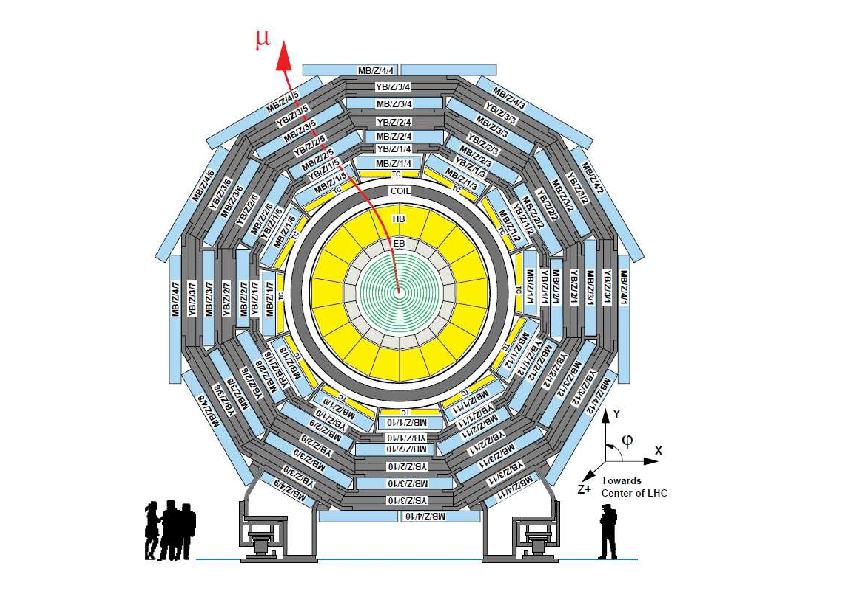
\includegraphics[width=0.45\textwidth]{../figs/Exp/CMSview.png}}
  \end{center}
\end{figure}
\end{frame}%{Compact Muon Solenoid (CMS). Components}


\begin{frame}\frametitle{Compact Muon Solenoid (CMS). Particle Reconstruction}
\scriptsize
Process to study: $W\gamma\rightarrow\mu\nu\gamma$, $W\gamma\rightarrow e\nu\gamma$.\\
Final state particles: muons, electrons, photons, neutrinos.\\
\begin{figure}[htb]
  \begin{center}
    {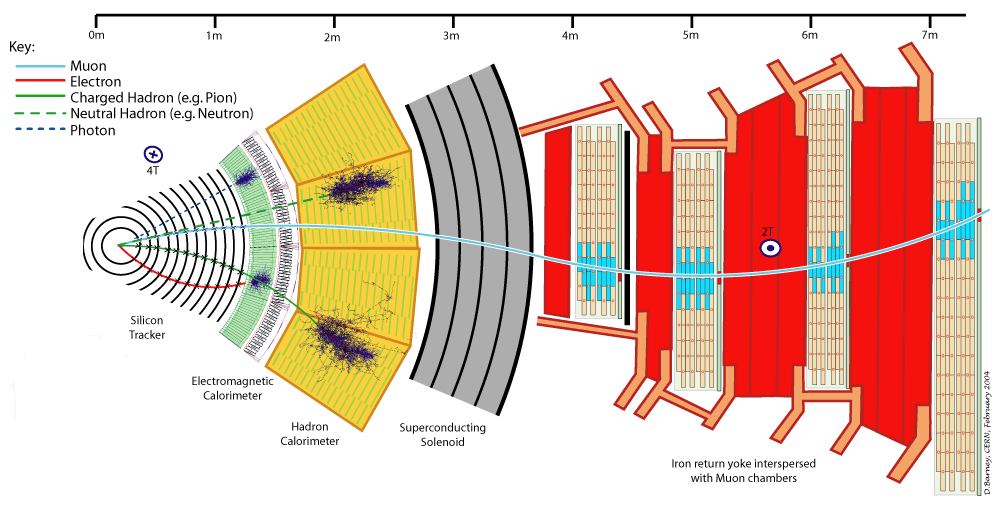
\includegraphics[width=0.75\textwidth]{../figs/Exp/CMS_Slice.png}}
  \end{center}
\end{figure}

\end{frame}%{Compact Muon Solenoid (CMS). Particle Reconstruction}

\begin{frame}\frametitle{Compact Muon Solenoid (CMS). Neutrinos}
\scriptsize
Process to study: $W\gamma\rightarrow\mu\nu\gamma$, $W\gamma\rightarrow e\nu\gamma$.\\
Final state particles: muons, electrons, photons, {\color{blue}\bfseries{neutrinos}}.\\
\begin{figure}[htb]
  \begin{center}
    {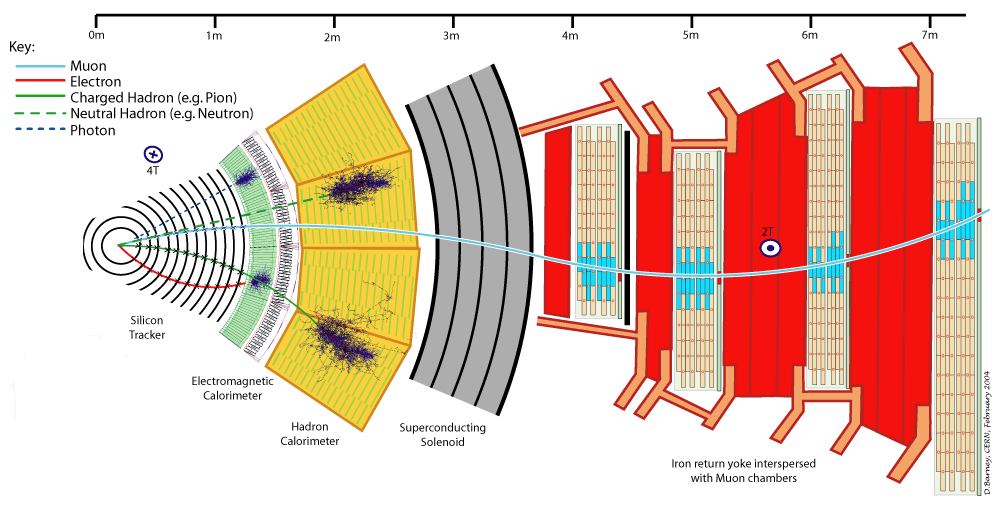
\includegraphics[width=0.45\textwidth]{../figs/Exp/CMS_Slice.png}}
  \end{center}
\end{figure}

\scriptsize
{\color{blue}\bfseries{Neutrino is not detected}}. The measure of $P_T^{\nu}$ is\\ 
{\bfseries{missing transverse energy}}: $  E_T^{miss} = - | \sum \mathbf{P_T} |$,\\
Sum over all visible particles in the event. 

\end{frame}%{Compact Muon Solenoid (CMS). Particle Reconstruction}


